\section{Analysis \& Discussion}

    \subsection{Known Issues}
    	In this section, known issues leading to improper or unexpected
    	behavior of the survey tool are discussed.

    	\subsubsection{Lack of Automated Tests}
    		No automated tests were written for this project. This proved
    		to be a major burden on development speed as the project
    		matured. When refactoring old code or adding new features,
    		tests help to identify potential problems at an early stage.
    		Without tests, bugs may be introduced into the codebase
    		without the maintainers noticing and may ultimately
    		affect the user in a negative way. Tests also
    		help to indentify conceptual inconsistencies
    		with new features more quickly. The codebase of the
    		backend is still relatively small, containing
    		approximately 5000 lines of Python. Test coverage for
    		the backend can still be achieved, but should be prioritized
    		over adding new features.

    	\subsubsection{Internationalisation of the User Interface}
    		While all user contributed content may be internationalized,
    		the user interface language itself is not yet dynamic.
    		Navigation and menus are all in English at the moment.
    		For the data client user interface, this is not as
    		problematic as for the data subject user interface, as 
    		currently, all data clients are associates of Prof. H. Drachsler.
    		For the data subject user interface, however, this is confusing,
    		as translated survey content is intermixed with
    		navigation elements in English.

    	\subsubsection{Edge Cases of the Template Management}
        \label{analysis:known-issues:template-management-edge-cases}
    		\begin{figure}
    			\centering
    			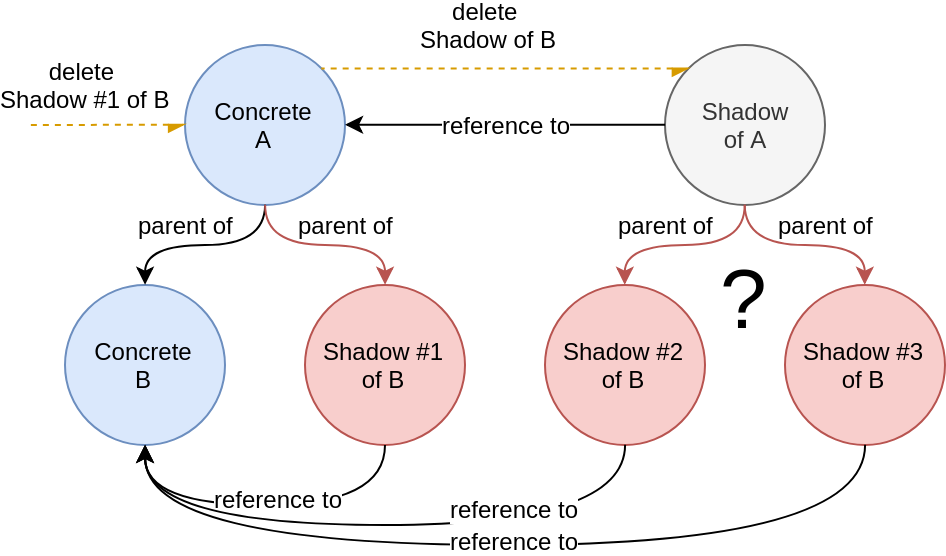
\includegraphics[width=.8\textwidth]{template-edge-case}
    			\caption{Using a shadow instance inside the source concrete breaks the delete action}
    			\label{fig:shadow-breaks-delete}
    		\end{figure}

    		When a shadow instance (Shadow \#1 of B) is created as a child of a concrete instance (Concrete A), which also contains the referenced
    		concrete instance (Concrete B) for the newly created shadow (Shadow \#1 of B), the following case may occur: when a shadow (Shadow of A) is created
    		of the parent instance, the relationship structure is also duplicated. The parent's shadow will
    		then end up with two child shadow instances (Shadow \#2 of B, Shadow \#3 of B), pointing to the same concrete child of the parent.
    		When trying to delete the original shadow instance (Shadow \#1 of B), the delete action is also propagated to all
    		shadows (Shadow of A) of its parent. Since these shadows now contain two copies of the
    		item to delete, there is no way of distinguishing which item to delete and the delete fails.
    		This edge case is depicted in Figure \ref{fig:shadow-breaks-delete}.
    		Since there exists no obvious use case for including the same survey item twice in a given survey,
    		this case is unlikely to occur during day-to-day usage of the survey tool.

    	\subsubsection{xAPI Statement Design}
    		A questionnaire is identified by its owner and its xAPI activity ID in xAPI statements.
    		When creating a questionnaire from a template, the shadow's xAPI activity ID will shadow
    		the template's xAPI activity ID for reasons described in Section \ref{section:concept:xapi-statement-design}.
    		This means that if a data client creates a shadow copy of their own
    		questionnaire, its xAPI activity ID will not be distinguishable from
    		the template's ID. The same case occurs, when a template is used multiple times
    		by a data client. A potential fix for this issue would be by
    		separating the xAPI activity ID from the user-configurable ID and
    		then generating the xAPI activity ID by concatenating information on
    		the owner, the user-configurable ID and the unique database ID
    		of the questionnaire. The resulting xAPI activity ID should be presented to the data client
    		in the user interface for reference.

    \subsection{Conceptual Issues}
    	In this section, issues with the concept of the survey tool are discussed.
    	These issues may not necessarily be critical to the operation of the tool,
    	but provide indications for future improvements.

	   	\subsubsection{xAPI Statement Design}
        \label{analysis:known-issues:xapi-not-normalized}
	   		In some places, the format of xAPI statements emitted by
	   		the survey tool is not completely normalized. This defeats
	   		the purpose of using the JSON format in the first place,
	   		as some fields have to be parsed a second time to extract all the
	   		data. The first case of this is the \inline{platform} string,
	   		which contains the name of the survey tool, as well as the
	   		LMS, which launched the survey tool. It would be more appropriate
	   		to include information about the LTI launch in the
	   		\inline{extensions} sections of the statement. For this,
	   		an extension for representing LTI launch information
	   		has to be drafted and specified.
	   		The second case is the activity ID used for representing
	   		survey items, which contains the owning data client's
	   		email address. This case is not as problematic, as the
	   		email address is only included to distinguish survey
	   		content owned by different data clients and not for
	   		reconstructing the data client from the ID.

		\subsubsection{OAuth \& The LTI Launch Protocol}
			It was not required to implement OAuth to secure
			access to the survey tool's LTI endpoint.
			This leaves the survey tool vulnerable to malicious
			launches by third parties. The combination of
			LTI endpoint and launch key used to launch the embedded
			user interface may be intercepted by using common
			network analysis tools included in every modern
			web browser. This data could then be used to construct
			a malicious launch request, allowing the attacker
			to be identified as a different or non-existent user.
			The solution to this issue is to implement OAuth
			as per the LTI specification.


    \subsection{Implementational Issues}
    	This section discusses cases, where the chosen implementation
    	of a certain feature is not optimal and may be improved in the
    	future.

    	\subsubsection{ORM Inheritance Mapping}
    		For mapping the survey tools class hierarchies to the database,
    		the joined table inheritance approach described in Section
    		\ref{section:implementation:inheritance-mapping} was used.
    		The reason given for this choice is storage optimization.
    		Storage, however, can easily be extended if required.
    		Access times cannot as easily be improved by upgrading the
    		underlying hardware. The joins produced by the joined table
    		inheritance approach usually use at least 3 tables in the
    		case of the survey tool. This can not be further optimized
    		with the current class hierarchies. Also, foreign key
    		constraints put in place by this approach require
    		careful configuration of delete and update cascades,
    		as modifications to one object instance might affect
    		all the tables along the object's inheritance chain.
    		Single table inheritance, despite lacking aesthetics,
    		is the more optimal approach for mapping class hierarchies,
    		if access times are prioritized over storage space used.

    	\subsubsection{Data Model}
    		The current data model used in the backend service does
    		not separate administrative data from survey content
    		in the \inline{Questionnaire}, \inline{Dimension} and
    		\inline{Question} classes. This makes it hard to separate
    		data (which should be visible to non-owners) from
    		sensitive data, which should only be visible to owners
    		of a survey item. Although this separation is already
    		enforced in the database as described in Section \ref{section:implementation:template-triad},
    		it is not consistently enforced throughout the backend service's
    		code. Separating survey content from administrative
    		data consistently throughout the codebase would
    		allow for better readability and -- by extension --
    		maintainability of the project.

        \subsubsection{Duplication of Functionality: Redis \& Memcached}
        	As described in Section \ref{section:implementation:architecture},
        	two different key-value stores, Redis and Memcached are used.
        	This is a leftover from prototyping. The backend service
        	has used Memcached since the previous version of the survey tool.
        	With the introduction of the xapi-publisher service and
        	the Celery library, a message broker had to be included
        	to distribute tasks to worker threads. Since Memcached
        	cannot be used for this purpose, Redis was included.
        	It is possible to completely replace the Memcached instance
        	by refactoring the backend service to use Redis instead.
        	This would result in less external dependencies and
     		is therefore favorable.

    \subsection{Conclusion}

    In conclusion, the research questions posed in the introduction of this
    thesis were answered, but additional questions for further research arise
    as well.

    The xAPI statement format suits itself well for data collection
    in the context of an online survey tool. As described in Section \ref{section:concept:xapi-statement-design},
    designing xAPI statements around the survey tool's use cases was
    straightforward. The level of detail provided by the format is
    more than sufficient for the application at hand. Because of the
    format's portability, special care needs to be taken when designing
    representations of objects. Adopters of the specification should
    be aware of the fact that a single identifier is often not sufficient
    for recognizing objects across systems, as no system is aware of all objects.
    The actor representations take this into account by combining a user identifier
    with an identifier of the domain which recognizes the user. The xAPI object does not yet
    provide a normalized representation for this. Adopters should also be aware
    of the fact, that depending on the source of an xAPI statement, the same person
    might be represented differently. To identify people in a reliable way,
    a list of all known representations of a person has to be maintained.
    How this can be achieved is a topic for future research.
    
    From a technical perspective, adoption of the xAPI specification is
    not particularly challenging, as it relies on widely used technologies.
    Special care needs to be taken with regards to transmission integrity,
    adopters should be aware that re-transmissions are required in case of
    network failure. Aggregation of xAPI statements and asynchronous transmission
    using a dedicated service, as described in Sections \ref{implementation:architecture:xapi-publisher}
    and \ref{implementation:xapi}, has worked well for this.

    Sharing of survey items between data clients can be achieved through
    the template management system described in Sections \ref{concept:template-management},
    \ref{section:implementation:template-triad} and \ref{implementation:template-management}.
    While the chosen approach is superior to simple import and export capabilities
    in the sense that it scales better and changes can be rolled out immediately 
    by authors of templates, it also introduced additional challenges.
    The biggest issue with he current system is that when a data client relies on a template,
    they do not have any control over changes to the content. Content might change
    at any time at the template author's discretion. This stifles trust in the reliability
    of templates. A content sharing system should therefore always include some sort
    of version control.

    For interoperability between the survey tool and the Moodle LMS, satisfying
    results have been achieved using the LTI launch protocol. The launch
    mechanism provides sufficient information for targeting specific resources
    the tool provider may provide to the LMS. Adopters of the specification
    should be aware that implementational details vary between LMS vendors.
    As discussed in Section \ref{section:concept:xapi-statement-design},
    some of the data provided in LTI requests might not be useful for a
    given application and vendor specific extensions may be in use.
    For these reasons, LTI launch requests may have to be handled
    differently by the tool provider depending on the launching LMS.